\chapter{Arhitektura i dizajn sustava}
		
		\textbf{\textit{dio 1. revizije}}\\

		\textit{ Potrebno je opisati stil arhitekture te identificirati: podsustave, preslikavanje na radnu platformu, spremišta podataka, mrežne protokole, globalni upravljački tok i sklopovsko-programske zahtjeve. Po točkama razraditi i popratiti odgovarajućim skicama:}
	\begin{itemize}
		\item 	\textit{izbor arhitekture temeljem principa oblikovanja pokazanih na predavanjima (objasniti zašto ste baš odabrali takvu arhitekturu)}
		\item 	\textit{organizaciju sustava s najviše razine apstrakcije (npr. klijent-poslužitelj, baza podataka, datotečni sustav, grafičko sučelje)}
		\item 	\textit{organizaciju aplikacije (npr. slojevi frontend i backend, MVC arhitektura) }		
	\end{itemize}

	
		

		

				
		\section{Baza podataka}

			Za potrebe naše aplikaicje korisiti ćemo relacijsku bazu podataka kako bismo lakše oblikovali stvarni svijet. Baza nam je potrbna za metodičku pohranu podataka te njihovo brzo dohvaćanje. Naša baza podataka se sastoji od sljedećih entiteta:
			
			\begin{packed_item}
				\item Patient
				\item Accommodation
				\item AccommodationOrder
				\item AccommodationBooking
				\item TransportCompany
				\item TransportVehicle
				\item TransportBooking
				\item MedicalAppointment
				\item AdminRole
				\item AdminRoles
				\item Admin
			\end{packed_item}
		
			\subsection{Opis tablica}
			

				\textit{Svaku tablicu je potrebno opisati po zadanom predlošku. Lijevo se nalazi točno ime varijable u bazi podataka, u sredini se nalazi tip podataka, a desno se nalazi opis varijable. Svjetlozelenom bojom označite primarni ključ. Svjetlo plavom označite strani ključ}
				\newline
				
				\noindent \text{\textbf{Patient} Ova tablica predstavlja}
				\begin{longtblr}[
					label=none,
					entry=none
					]{
						width = \textwidth,
						colspec={|X[6,l]|X[6, l]|X[20, l]|}, 
						rowhead = 1,
					} %definicija širine tablice, širine stupaca, poravnanje i broja redaka naslova tablice
				
					\hline 
					\SetCell[c=3]{c}{\textbf{Patient}}\\
					\hline[3pt]
					\SetCell{LightGreen}patient\_ID & VARCHAR & primarni ključ tablice \\
					\hline
					first\_name	& VARCHAR &  ime pacijenta\\ 
					\hline 
					last\_name & VARCHAR &  prezime pacijenta \\ 
					\hline 
					PIN & VARCHAR	&  Personal Identification Number, kao OIB u hrvatskoj\\ 
					\hline 
					email & VARCHAR & pacijentov email\\ 
					\hline	
					phone\_number & VARCHAR & pacijentov telefonski broj \\
					\hline
				\end{longtblr}
				
				\begin{longtblr}[
					label=none,
					entry=none
					]{
						width = \textwidth,
						colspec={|X[6,l]|X[6, l]|X[20, l]|}, 
						rowhead = 1,
					} %definicija širine tablice, širine stupaca, poravnanje i broja redaka naslova tablice
					\hline 
					\SetCell[c=3]{c}{\textbf{korisnik - ime tablice}}\\ 
					\hline[3pt]
					\SetCell{LightGreen}PK & type & \\ 
					\hline
					fieldName & type & opis \\
					\hline 
					\SetCell{LightBlue} FK	& type & opis \\
					\hline 
				\end{longtblr}
				
				
			
			\subsection{Dijagram baze podataka}

				\begin{figure}[H]
					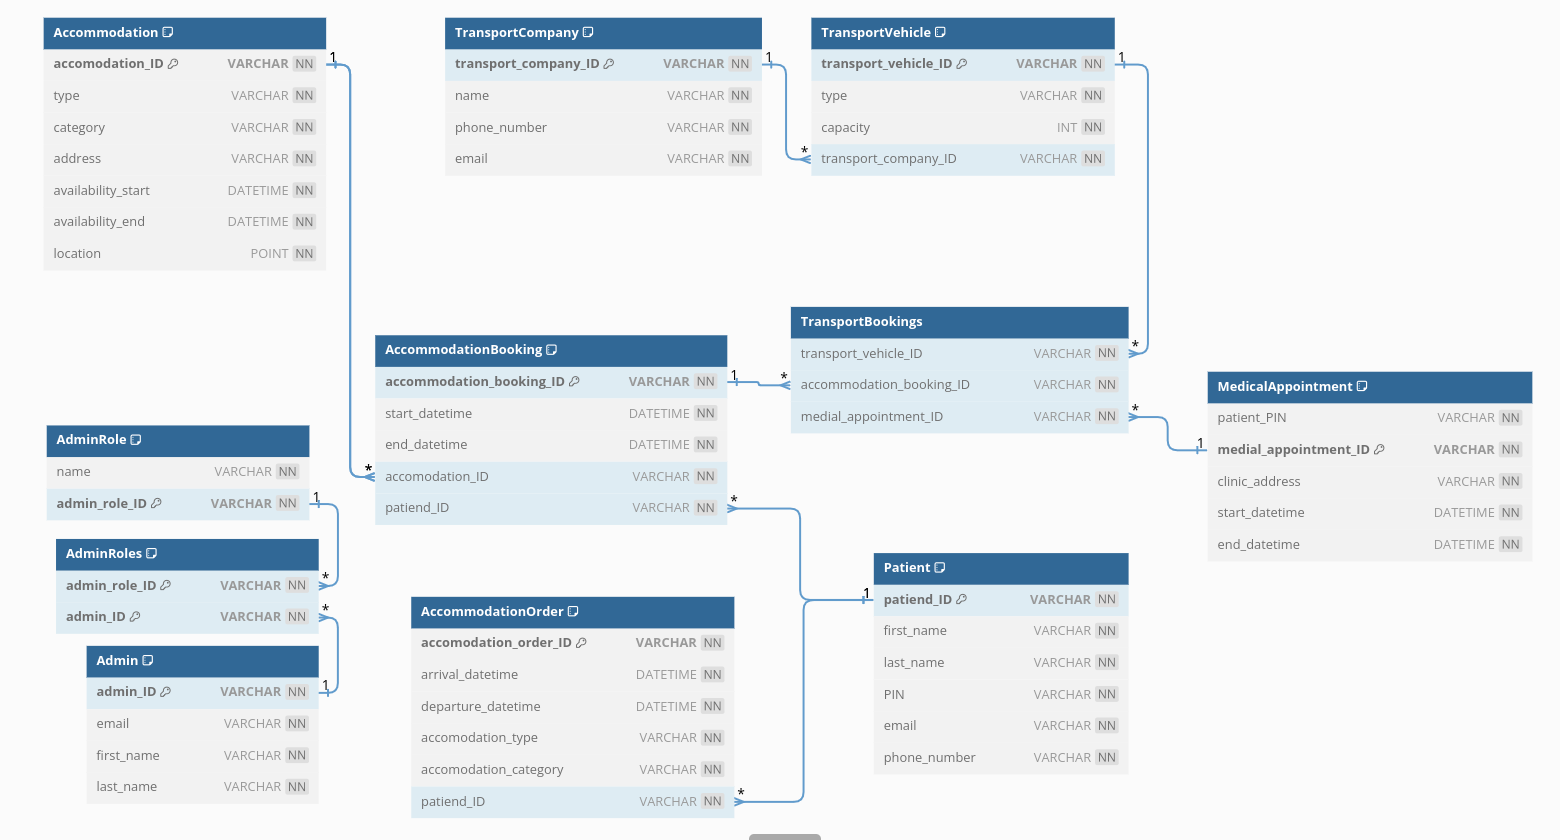
\includegraphics[scale=0.32]{slike/dijagram_baze.png} %veličina slike u odnosu na originalnu datoteku i pozicija slike
					\centering
					\caption{ER Dijagram baze podataka}
					\label{fig:dijagram_baze_podataka}
				\end{figure}
			
			\eject
			
			
		\section{Dijagram razreda}
		
			\textit{Potrebno je priložiti dijagram razreda s pripadajućim opisom. Zbog preglednosti je moguće dijagram razlomiti na više njih, ali moraju biti grupirani prema sličnim razinama apstrakcije i srodnim funkcionalnostima.}\\
			
			\textbf{\textit{dio 1. revizije}}\\
			
			\textit{Prilikom prve predaje projekta, potrebno je priložiti potpuno razrađen dijagram razreda vezan uz \textbf{generičku funkcionalnost} sustava. Ostale funkcionalnosti trebaju biti idejno razrađene u dijagramu sa sljedećim komponentama: nazivi razreda, nazivi metoda i vrste pristupa metodama (npr. javni, zaštićeni), nazivi atributa razreda, veze i odnosi između razreda.}\\
			
			\textbf{\textit{dio 2. revizije}}\\			
			
			\textit{Prilikom druge predaje projekta dijagram razreda i opisi moraju odgovarati stvarnom stanju implementacije}
			
			
			
			\eject
		
		\section{Dijagram stanja}
			
			
			\textbf{\textit{dio 2. revizije}}\\
			
			\textit{Potrebno je priložiti dijagram stanja i opisati ga. Dovoljan je jedan dijagram stanja koji prikazuje \textbf{značajan dio funkcionalnosti} sustava. Na primjer, stanja korisničkog sučelja i tijek korištenja neke ključne funkcionalnosti jesu značajan dio sustava, a registracija i prijava nisu. }
			
			
			\eject 
		
		\section{Dijagram aktivnosti}
			
			\textbf{\textit{dio 2. revizije}}\\
			
			 \textit{Potrebno je priložiti dijagram aktivnosti s pripadajućim opisom. Dijagram aktivnosti treba prikazivati značajan dio sustava.}
			
			\eject
		\section{Dijagram komponenti}
		
			\textbf{\textit{dio 2. revizije}}\\
		
			 \textit{Potrebno je priložiti dijagram komponenti s pripadajućim opisom. Dijagram komponenti treba prikazivati strukturu cijele aplikacije.}